
\documentclass{article}
\usepackage[utf8]{inputenc}
\usepackage[english]{babel}
\usepackage[]{amsthm} %lets us use \begin{proof}
\usepackage[]{amssymb} %gives us the character \varnothing
\usepackage[]{setspace} %provides commands to set line spacing
\usepackage[left=0.75in, right=0.75in]{geometry}
\usepackage{hyperref}
\usepackage{xcolor}
\usepackage{soul}
\usepackage{amsmath}
\usepackage{amsfonts} % for \mathbb
\usepackage{amssymb}
\usepackage{graphicx}
\usepackage{float}





\begin{document}

\begin{center}
	\LARGE{Ansatz}\\[1em]
	\large Son Nguyen\\[1em]
	%\large \today
\end{center}

\subsubsection*{Example:}
We start with defining the Hamiltonian of of the molecular Hydgrogen.
\[H = g_0 \mathbb{I} + g_1 Z_0 + g_2 Z_1 + g_3 Z_0 Z_1 + g_4 Y_0 Y_1 + g_5 X_0 X_ 1\]
Where: $\{X_i, Z_i, Y_i\}$ denote the Pauli matrices acting on the i-th qubit and the real scalars $\{g_\gamma\}$ are efficiently computable functions of the hydrogen-hydrogen bond length R.
\[
	X = \begin{bmatrix}
		0 & 1 \\
		1 & 0
	\end{bmatrix} , \quad
	\mathbb{I} = \begin{bmatrix}
		1 & 0 \\
		0 & 1
	\end{bmatrix}, \quad
	Y = \begin{bmatrix}
		0 & -i \\
		i & 0
	\end{bmatrix}, \quad
	Z = \begin{bmatrix}
		1 & 0  \\
		0 & -1
	\end{bmatrix}
\]
\[g_0 \mathbb{I} = \begin{bmatrix}
		g_0 & 0   & 0   & 0   \\
		0   & g_0 & 0   & 0   \\
		0   & 0   & g_0 & 0   \\
		0   & 0   & 0   & g_0
	\end{bmatrix}, \quad
	g_1 Z_0 = \begin{bmatrix}
		g_1 & 0   & 0    & 0    \\
		0   & g_1 & 0    & 0    \\
		0   & 0   & -g_1 & 0    \\
		0   & 0   & 0    & -g_1
	\end{bmatrix}, \quad
	g_2 Z_1 = \begin{bmatrix}
		g_2 & 0    & 0   & 0    \\
		0   & -g_2 & 0   & 0    \\
		0   & 0    & g_2 & 0    \\
		0   & 0    & 0   & -g_2
	\end{bmatrix}, \quad
\]
\\
\[
	g_3 Z_0 Z_1 = \begin{bmatrix}
		g_3 & 0    & 0    & 0   \\
		0   & -g_3 & 0    & 0   \\
		0   & 0    & -g_3 & 0   \\
		0   & 0    & 0    & g_3
	\end{bmatrix}, \quad
	g_4 Y_0 Y_1 = \begin{bmatrix}
		0   & 0  & 0  & -g4 \\
		0   & 0  & g4 & 0   \\
		0   & g4 & 0  & 0   \\
		-g4 & 0  & 0  & 0
	\end{bmatrix}, \quad
	g_5 X_0 X_1 = \begin{bmatrix}
		0  & 0  & 0  & g5 \\
		0  & 0  & g5 & 0  \\
		0  & g5 & 0  & 0  \\
		g5 & 0  & 0  & 0
	\end{bmatrix}
\]
\\
\[
	H = \begin{bmatrix}
		g_0 + g_1 + g_2 + g_3 & 0                     & 0                     & g_5 - g_4              \\
		0                     & g_0 + g_1 - g_2 - g_3 & g_5 + g_4             & 0                      \\
		0                     & g_5 + g_4             & g_0 - g_1 + g_2 - g_3 & 0                      \\
		g_5 - g_4             & 0                     & 0                     & g_0 - g_1 - g_2 +  g_3
	\end{bmatrix}
\]
\subsubsection*{Decomposing the UCCSD ansatz}
\begin{figure}[h]
	\centering
	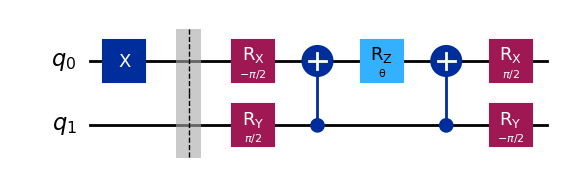
\includegraphics[width=0.8\textwidth, height=0.2\textheight]{Circ.png}
	\caption{The UCCSD ansatz for the Hydrogen molecule.}
	\label{fig:yourlabel}
\end{figure}
\begin{itemize}
	\item Reference state \(|10 \rangle\)
	      \begin{figure}[H]
		      \centering
		      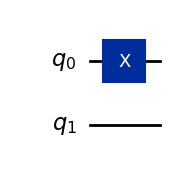
\includegraphics[width=0.2\textwidth, height=0.2\textheight]{ref.png}
	      \end{figure}
	      \[
		      \left( X \otimes I\right) \cdot \left( |0 \rangle \otimes | 0 \rangle \right) = |10 \rangle
	      \]
	      \[
		      \left(
		      \begin{bmatrix}
				      0 & 1 \\
				      1 & 0
			      \end{bmatrix}
		      \otimes
		      \begin{bmatrix}
				      1 & 0 \\
				      0 & 1
			      \end{bmatrix}
		      \right)
		      \cdot
		      \left(
		      \begin{bmatrix}
				      1 \\
				      0
			      \end{bmatrix}
		      \otimes
		      \begin{bmatrix}
				      1 \\
				      0
			      \end{bmatrix}
		      \right)
		      =
		      \begin{bmatrix}
			      0 \\
			      0 \\
			      1 \\
			      0
		      \end{bmatrix}
	      \]

	\item Apply parameterized ansatz
	      \begin{figure}[H]
		      \centering
		      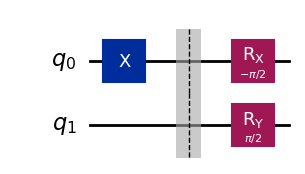
\includegraphics[width=0.3\textwidth, height=0.15\textheight]{ansatz1.png}
	      \end{figure}
	      \[
		      \left(R_x(\frac{-\pi}{2}) \otimes R_y(\frac{\pi}{2})\right) \cdot |10 \rangle
	      \]

	      \[
		      R_x(\frac{-\pi}{2}) = e^{-i X (\frac{-\pi}{4})} = \begin{bmatrix}
			      \cos(\frac{-\pi}{4})   & -i\sin(\frac{-\pi}{4}) \\
			      -i\sin(\frac{-\pi}{4}) & \cos(-\frac{\pi}{4})
		      \end{bmatrix}
		      =
		      \begin{bmatrix}
			      \frac{\sqrt{2}}{2}   & \frac{i \sqrt{2}}{2} \\
			      \frac{i \sqrt{2}}{2} & \frac{\sqrt{2}}{2}
		      \end{bmatrix}
	      \]

	      \[
		      R_y(\frac{\pi}{2}) = e^{ -i Y(\frac{\pi}{4})} =
		      \begin{bmatrix}
			      \cos(\frac{\pi}{4}) & -\sin(\frac{\pi}{4}) \\
			      \sin(\frac{\pi}{4}) & \cos(\frac{\pi}{4})
		      \end{bmatrix} =
		      \begin{bmatrix}
			      \frac{\sqrt{2}}{2} & -\frac{\sqrt{2}}{2} \\
			      \frac{\sqrt{2}}{2} & \frac{\sqrt{2}}{2}
		      \end{bmatrix}
	      \]

	      \[
		      \left(R_x(\frac{-\pi}{2}) \otimes R_y(\frac{\pi}{2})\right) =
		      \begin{bmatrix}
			      \frac{\sqrt{2}}{2}   & \frac{i \sqrt{2}}{2} \\
			      \frac{i \sqrt{2}}{2} & \frac{\sqrt{2}}{2}
		      \end{bmatrix}
		      \otimes
		      \begin{bmatrix}
			      \frac{\sqrt{2}}{2} & -\frac{\sqrt{2}}{2} \\
			      \frac{\sqrt{2}}{2} & \frac{\sqrt{2}}{2}
		      \end{bmatrix} =
		      \begin{bmatrix}
			      \frac{1}{2} & \frac{-1}{2} & \frac{i}{2} & \frac{-i}{2} \\
			      \frac{1}{2} & \frac{1}{2}  & \frac{i}{2} & \frac{i}{2}  \\
			      \frac{i}{2} & \frac{-i}{2} & \frac{1}{2} & \frac{-1}{2} \\
			      \frac{i}{2} & \frac{i}{2}  & \frac{1}{2} & \frac{1}{2}
		      \end{bmatrix}
	      \]

	      \[
		      \left(R_x(\frac{-\pi}{2}) \otimes R_y(\frac{\pi}{2})\right) \cdot |10 \rangle =
		      \begin{bmatrix}
			      \frac{1}{2} & \frac{-1}{2} & \frac{i}{2} & \frac{-i}{2} \\
			      \frac{1}{2} & \frac{1}{2}  & \frac{i}{2} & \frac{i}{2}  \\
			      \frac{i}{2} & \frac{-i}{2} & \frac{1}{2} & \frac{-1}{2} \\
			      \frac{i}{2} & \frac{i}{2}  & \frac{1}{2} & \frac{1}{2}
		      \end{bmatrix}
		      \cdot
		      \begin{bmatrix}
			      0 \\
			      0 \\
			      1 \\
			      0
		      \end{bmatrix}
		      =
		      \begin{bmatrix}
			      \frac{i}{2} \\
			      \frac{i}{2} \\
			      \frac{1}{2} \\
			      \frac{1}{2} \\
		      \end{bmatrix}
	      \]
	      The first CNOT (entanglement)
	      \begin{figure}[H]
		      \centering
		      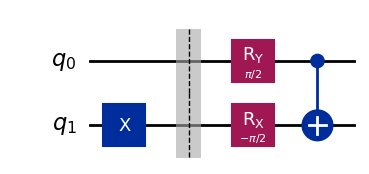
\includegraphics[width=0.3\textwidth, height=0.15\textheight]{1cnot.png}

	      \end{figure}
	      \[
		      \begin{bmatrix}
			      1 & 0 & 0 & 0 \\
			      0 & 0 & 0 & 1 \\
			      0 & 0 & 1 & 0 \\
			      0 & 1 & 0 & 0
		      \end{bmatrix}
		      \cdot
		      \begin{bmatrix}
			      \frac{i}{2} \\
			      \frac{i}{2} \\
			      \frac{1}{2} \\
			      \frac{1}{2} \\
		      \end{bmatrix}
		      =
		      \begin{bmatrix}
			      \frac{i}{2} \\
			      \frac{1}{2} \\
			      \frac{1}{2} \\
			      \frac{i}{2} \\
		      \end{bmatrix}
	      \]
	      The \(Z_\theta\) rotation gate:
	      \[
		      Z_\theta = e^{-iZ(\frac{\theta}{2})} =
		      \begin{bmatrix}
			      e^{-i \frac{\theta}{2}} & 0                      \\
			      0                       & e^{i \frac{\theta}{2}}
		      \end{bmatrix}
	      \]

	      \[
		      (Z_\theta \otimes I) \cdot \begin{bmatrix}
			      \frac{i}{2} \\
			      \frac{1}{2} \\
			      \frac{1}{2} \\
			      \frac{i}{2} \\
		      \end{bmatrix} =
		      \begin{bmatrix}
			      e^{-i \frac{\theta}{2}} & 0                       & 0                      & 0                      \\
			      0                       & e^{-i \frac{\theta}{2}} & 0                      & 0                      \\
			      0                       & 0                       & e^{i \frac{\theta}{2}} & 0                      \\
			      0                       & 0                       & 0                      & e^{i \frac{\theta}{2}}
		      \end{bmatrix}
		      \cdot
		      \begin{bmatrix}
			      \frac{i}{2} \\
			      \frac{1}{2} \\
			      \frac{1}{2} \\
			      \frac{i}{2} \\
		      \end{bmatrix} =
		      \begin{bmatrix}
			      \frac{\sin \left(\frac{\theta}{2}\right)}{2} + i \frac{\cos \left(\frac{\theta}{2}\right)}{2} \\
			      \frac{\cos \left(\frac{\theta}{2}\right)}{2} - i \frac{\sin \left(\frac{\theta}{2}\right)}{2} \\
			      \frac{\cos \left(\frac{\theta}{2}\right)}{2} + i \frac{\sin \left(\frac{\theta}{2}\right)}{2} \\
			      \frac{-\sin \left(\frac{\theta}{2}\right)}{2} + i \frac{\cos \left(\frac{\theta}{2}\right)}{2}
		      \end{bmatrix}
	      \]
	      The second CNOT (entanglement)
	      \[
		      \begin{bmatrix}
			      1 & 0 & 0 & 0 \\
			      0 & 0 & 0 & 1 \\
			      0 & 0 & 1 & 0 \\
			      0 & 1 & 0 & 0
		      \end{bmatrix}
		      \cdot
		      \begin{bmatrix}
			      \frac{\sin \left(\frac{\theta}{2}\right)}{2} + i \frac{\cos \left(\frac{\theta}{2}\right)}{2} \\
			      \frac{\cos \left(\frac{\theta}{2}\right)}{2} - i \frac{\sin \left(\frac{\theta}{2}\right)}{2} \\
			      \frac{\cos \left(\frac{\theta}{2}\right)}{2} + i \frac{\sin \left(\frac{\theta}{2}\right)}{2} \\
			      \frac{-\sin \left(\frac{\theta}{2}\right)}{2} + i \frac{\cos \left(\frac{\theta}{2}\right)}{2}
		      \end{bmatrix}
		      =
		      \begin{bmatrix}
			      \frac{\sin \left(\frac{\theta}{2}\right)}{2} + i \frac{\cos \left(\frac{\theta}{2}\right)}{2}  \\
			      \frac{-\sin \left(\frac{\theta}{2}\right)}{2} + i \frac{\cos \left(\frac{\theta}{2}\right)}{2} \\
			      \frac{\cos \left(\frac{\theta}{2}\right)}{2} + i \frac{\sin \left(\frac{\theta}{2}\right)}{2}  \\
			      \frac{\cos \left(\frac{\theta}{2}\right)}{2} - i \frac{\sin \left(\frac{\theta}{2}\right)}{2}
		      \end{bmatrix}
	      \]
	      The final rotation gates:
	      \[\left(R_x(\frac{\pi}{2}) \otimes R_y(\frac{-\pi}{2})\right) \cdot
		      \begin{bmatrix}
			      \frac{\sin \left(\frac{\theta}{2}\right)}{2} + i \frac{\cos \left(\frac{\theta}{2}\right)}{2}  \\
			      \frac{-\sin \left(\frac{\theta}{2}\right)}{2} + i \frac{\cos \left(\frac{\theta}{2}\right)}{2} \\
			      \frac{\cos \left(\frac{\theta}{2}\right)}{2} + i \frac{\sin \left(\frac{\theta}{2}\right)}{2}  \\
			      \frac{\cos \left(\frac{\theta}{2}\right)}{2} - i \frac{\sin \left(\frac{\theta}{2}\right)}{2}
		      \end{bmatrix}
	      \]

	      \[
		      =
		      \left(
		      \begin{bmatrix}
				      \cos \left(\frac{\pi}{4}\right)    & -i \sin \left(\frac{\pi}{4}\right) \\
				      -i \sin \left(\frac{\pi}{4}\right) & \cos \left(\frac{\pi}{4}\right)
			      \end{bmatrix}
		      \otimes
		      \begin{bmatrix}
				      \cos \left(\frac{-\pi}{4}\right) & - \sin \left(\frac{-\pi}{4}\right) \\
				      \sin \left(\frac{-\pi}{4}\right) & \cos \left(\frac{-\pi}{4}\right)
			      \end{bmatrix}
		      \right)
		      \cdot
		      \begin{bmatrix}
			      \frac{\sin \left(\frac{\theta}{2}\right)}{2} + i \frac{\cos \left(\frac{\theta}{2}\right)}{2}  \\
			      \frac{-\sin \left(\frac{\theta}{2}\right)}{2} + i \frac{\cos \left(\frac{\theta}{2}\right)}{2} \\
			      \frac{\cos \left(\frac{\theta}{2}\right)}{2} + i \frac{\sin \left(\frac{\theta}{2}\right)}{2}  \\
			      \frac{\cos \left(\frac{\theta}{2}\right)}{2} - i \frac{\sin \left(\frac{\theta}{2}\right)}{2}
		      \end{bmatrix}
	      \]

	      \[
		      =
		      \left(
		      \begin{bmatrix}
				      \frac{1}{\sqrt{2}}  & \frac{-i}{\sqrt{2}} \\
				      \frac{-i}{\sqrt{2}} & \frac{1}{\sqrt{2}}
			      \end{bmatrix}
		      \otimes
		      \begin{bmatrix}
				      \frac{1}{\sqrt{2}}  & \frac{1}{\sqrt{2}} \\
				      \frac{-1}{\sqrt{2}} & \frac{1}{\sqrt{2}}
			      \end{bmatrix}
		      \right)
		      \cdot
		      \begin{bmatrix}
			      \frac{\sin \left(\frac{\theta}{2}\right)}{2} + i \frac{\cos \left(\frac{\theta}{2}\right)}{2}  \\
			      \frac{-\sin \left(\frac{\theta}{2}\right)}{2} + i \frac{\cos \left(\frac{\theta}{2}\right)}{2} \\
			      \frac{\cos \left(\frac{\theta}{2}\right)}{2} + i \frac{\sin \left(\frac{\theta}{2}\right)}{2}  \\
			      \frac{\cos \left(\frac{\theta}{2}\right)}{2} - i \frac{\sin \left(\frac{\theta}{2}\right)}{2}
		      \end{bmatrix}
	      \]

	      \begin{equation}
		      \label{eq:1}
		      =
		      \begin{bmatrix}
			      \frac{1}{2}  & \frac{1}{2}  & \frac{-i}{2} & \frac{-i}{2} \\
			      \frac{-1}{2} & \frac{1}{2}  & \frac{i}{2}  & \frac{-i}{2} \\
			      \frac{-i}{2} & \frac{-i}{2} & \frac{1}{2}  & \frac{1}{2}  \\
			      \frac{i}{2}  & \frac{-i}{2} & \frac{-1}{2} & \frac{1}{2}
		      \end{bmatrix}
		      \cdot
		      \begin{bmatrix}
			      \frac{\sin \left(\frac{\theta}{2}\right)}{2} + i \frac{\cos \left(\frac{\theta}{2}\right)}{2}  \\
			      \frac{-\sin \left(\frac{\theta}{2}\right)}{2} + i \frac{\cos \left(\frac{\theta}{2}\right)}{2} \\
			      \frac{\cos \left(\frac{\theta}{2}\right)}{2} + i \frac{\sin \left(\frac{\theta}{2}\right)}{2}  \\
			      \frac{\cos \left(\frac{\theta}{2}\right)}{2} - i \frac{\sin \left(\frac{\theta}{2}\right)}{2}
		      \end{bmatrix}
		      =
		      \begin{bmatrix}
			      0                        \\
			      - \sin(\frac{\theta}{2}) \\
			      \cos(\frac{\theta}{2})   \\
			      0
		      \end{bmatrix}
		      = |\phi(\vec{\theta}) \rangle = -\sin\left(\frac{\theta}{2}\right) |01 \rangle + \cos\left(\frac{\theta}{2}\right) |10 \rangle
	      \end{equation}
	      \textbf{*Note: the first qubit is the left most bit.}

	\item The expectation value (Quantum Tomography):
	      \hl{Using many measurements on identically prepared systems to get mean values of the some complete set of observables to reconstruct an estimate of the state. Quantum Tomography works to
		      determine the state prior to the measurements.}

	      In this case, our state we want to reconstruct is \(|\phi(\vec{\theta})\rangle\).
	      \\
	      Starting with the denstiy matrix:
	      \begin{equation*}
		      \rho = |\phi(\vec{\theta})\rangle \langle \phi(\vec{\theta})|
	      \end{equation*}
	      The general two qubits wavefunction can be written as:
	      \begin{equation*}
		      | \phi \rangle = a_{00} |00\rangle + a_{01} |01\rangle + a_{10} |10\rangle + a_{11} |11\rangle
	      \end{equation*}
	      Where \(a_{ij} \in \mathbb{C}\), and \(\sum_{i,j} |a_{ij}|^2 = 1\). For our case, we have:
            \begin{equation*}
                | \phi(\vec{\theta}) \rangle = -\sin\left(\frac{\theta}{2}\right) |01\rangle + \cos\left(\frac{\theta}{2}\right) |10\rangle
            \end{equation*}
            Where: \(a_{00} = 0, a_{01} = -\sin\left(\frac{\theta}{2}\right), a_{10} = \cos\left(\frac{\theta}{2}\right), a_{11} = 0 \), the goal is to reconstruct
            \(a_{01}\) and \(a_{10}\). To achieve this, we need to make measurement in different basis. (X, Y, Z). 

            To be countinue...
	      \\ \\
    \item Alternatively, using Bell Measurement to reconstruct the trial wavefunction with the parameter \(\theta \approx -3.37\), getting the expectation after 1000 measurements:
	      \begin
	      {figure}[H]
	      \centering
	      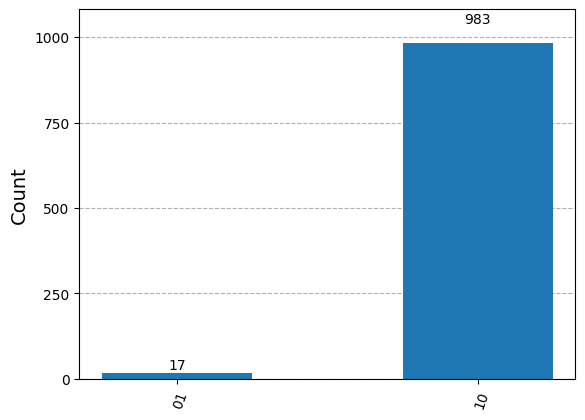
\includegraphics[width=0.5\textwidth, height=0.3\textheight]{1000.png}
	      \end{figure}

	      From the figure, we have see there is \(1.7 \% \) of \(|01\rangle\) and \(98.3 \%\) of \(|10\rangle\).
	      \begin{align*}
		      \sqrt{98.3 \%}|01\rangle +\sqrt{1.7 \% } |10\rangle & = |\phi(\vec{\theta}) \rangle \\
		      \pm 0.99 |01\rangle \pm 0.13 |10\rangle             & = |\phi(\vec{\theta}) \rangle
	      \end{align*}
	      To determine the sign of our trial wavefunction, we can use Bell measurements. We can measures any state which is an superposition of \(|00\rangle, |01\rangle, |10\rangle , |11\rangle\) in the Bell basis.
	      \begin{align*}
		      |\Phi^+\rangle & = \frac{1}{\sqrt{2}}(|00\rangle + |11\rangle) \\
		      |\Phi^-\rangle & = \frac{1}{\sqrt{2}}(|00\rangle - |11\rangle) \\
		      |\Psi^+\rangle & = \frac{1}{\sqrt{2}}(|01\rangle + |10\rangle) \\
		      |\Psi^-\rangle & = \frac{1}{\sqrt{2}}(|01\rangle - |10\rangle)
	      \end{align*}
	      By combining a CNOT gate followed by a Hadamard gate, we can measure the state in the Bell basis.
	      \begin{align*}
		      U |\Phi^+\rangle & = |00\rangle \\
		      U |\Phi^-\rangle & = |01\rangle \\
		      U |\Psi^+\rangle & = |10\rangle \\
		      U |\Psi^-\rangle & = |11\rangle
	      \end{align*}
	      Where \(U_{Bell} = \left( H \otimes I \right) \cdot \text{CNOT}(0,1)\)
	      \begin{equation*}
		      U_{Bell} = \frac{1}{\sqrt{2}}\begin{bmatrix}
			      1 & 0 & 0  & 1  \\
			      0 & 1 & 1  & 0  \\
			      1 & 0 & 0  & -1 \\
			      0 & 1 & -1 & 0
		      \end{bmatrix}
	      \end{equation*}
	      Applying the \(U_{Bell}\) on \(\begin{bmatrix}
		      A \\
		      B \\
		      C \\
		      D
	      \end{bmatrix}\)
	      \begin{equation*}
		      U_{Bell} \cdot \begin{bmatrix}
			      A \\
			      B \\
			      C \\
			      D
		      \end{bmatrix}
		      =
		      \frac{1}{\sqrt{2}}\begin{bmatrix}
			      A + D \\
			      B + C \\
			      A - D \\
			      B - C
		      \end{bmatrix}
	      \end{equation*}
	      \begin{figure}[H]
		      \centering
		      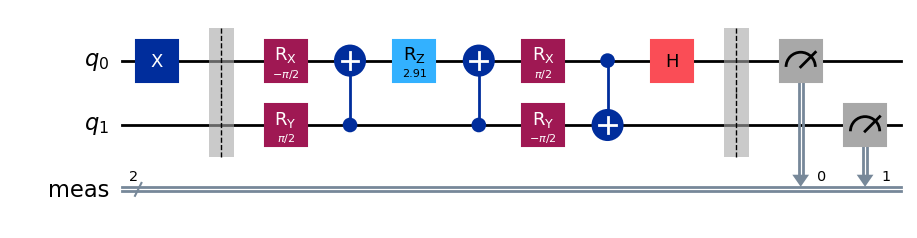
\includegraphics[width=0.9\textwidth, height=0.25\textheight]{BellM.png}
	      \end{figure}
	      The trial wavefunction after applying the \(U_{Bell}\) unitary gate:
	      \begin{equation*}
		      U_{Bell} \cdot |\phi(\vec{\theta})\rangle = U_{Bell} \cdot \begin{bmatrix}
			      0                                  \\
			      -\sin\left(\frac{\theta}{2}\right) \\
			      \cos\left(\frac{\theta}{2}\right)  \\
			      0
		      \end{bmatrix}
		      = \frac{1}{\sqrt{2}}
		      \begin{bmatrix}
			      0                                                                     \\
			      \cos\left(\frac{\theta}{2}\right) - \sin\left(\frac{\theta}{2}\right) \\
			      0                                                                     \\
			      -\cos\left(\frac{\theta}{2}\right) - \sin\left(\frac{\theta}{2}\right)
		      \end{bmatrix}
		      \begin{array}{c}
			      |00 \rangle \\
			      |01 \rangle \\
			      |10 \rangle \\
			      |11 \rangle
		      \end{array}
		      \begin{array}{c}
			      \\
			      \approx 0.39\% \\
			      \\
			      \approx 0.61\%
		      \end{array}
	      \end{equation*}
	      Using \(\theta \approx -3.37\) we have:
	      \begin{figure}[H]
		      \centering
		      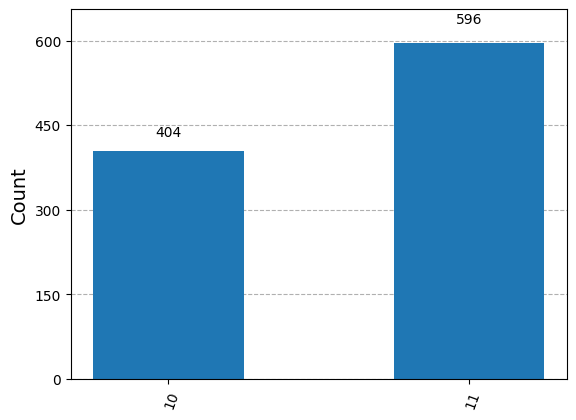
\includegraphics[width=0.5\textwidth, height=0.3\textheight]{BellHis.png}
	      \end{figure}
	      We can see the counts of \(|11\rangle\) is dominant, which means the state is \(|\Psi^-\rangle\). Therefore, the sign between \(|01\rangle\) and \(|10\rangle\) is negative.
	      \begin{equation}
		      0.99 |01\rangle - 0.13 |10\rangle = |\phi(\vec{\theta}) \rangle
	      \end{equation}

	      \href{https://grishmaprs.medium.com/measurement-based-quantum-computation-9de426f40856}{\hl{Reference}}.


	      Now we plug in the \(\theta\) to equation \eqref{eq:1} to compare with equation (2), we have:
	      \begin{align*}
		      -\sin\left(\frac{-3.37}{2}\right) |01 \rangle + \cos\left(\frac{-3.37}{2}\right) |10 \rangle & = |\phi(\vec{\theta}) \rangle \\
		      0.993 |01\rangle  - 0.11 |10\rangle                                                          & = |\phi(\vec{\theta}) \rangle
	      \end{align*}
	      Mathematically we can use the Hamiltonian and the trial wavefunction, we can get our cost function (energy) as:
	      \[E = \langle \phi({\vec{\theta}})| H | \phi(\vec{\theta}) \rangle\]
	      \[
		      \begin{bmatrix}
			      0 & -\sin(\frac{\theta}{2}) & \cos(\frac{\theta}{2}) & 0
		      \end{bmatrix}
		      \cdot
		      \begin{bmatrix}
			      g_0 + g_1 + g_2 + g_3 & 0                     & 0                     & g_5 - g_4              \\
			      0                     & g_0 + g_1 - g_2 - g_3 & g_5 + g_4             & 0                      \\
			      0                     & g_5 + g_4             & g_0 - g_1 + g_2 - g_3 & 0                      \\
			      g_5 - g_4             & 0                     & 0                     & g_0 - g_1 - g_2 +  g_3
		      \end{bmatrix}
		      \cdot
		      \begin{bmatrix}
			      0                        \\
			      - \sin(\frac{\theta}{2}) \\
			      \cos(\frac{\theta}{2})   \\
			      0
		      \end{bmatrix}
	      \]

	      Plug in  \(g_0 = -0.4804, g_1 = 0.3435, g_2 = -0.4347, g_3 = 0.5716, g_4 = 0.091, g_5 = 0.091\) we have:
	      \[
		      \begin{bmatrix}
			      0 & -\sin(\frac{\theta}{2}) & \cos(\frac{\theta}{2}) & 0
		      \end{bmatrix}
		      \cdot
		      \begin{bmatrix}
			      0 & 0       & 0       & 0      \\
			      0 & -0.2738 & 0.182   & 0      \\
			      0 & 0.182   & -1.8302 & 0      \\
			      0 & 0       & 0       & 0.1824
		      \end{bmatrix}
		      \cdot
		      \begin{bmatrix}
			      0                        \\
			      - \sin(\frac{\theta}{2}) \\
			      \cos(\frac{\theta}{2})   \\
			      0
		      \end{bmatrix}
	      \]

	      \[
		      \begin{bmatrix}
			      0 & \frac{910 \cdot \cos\left(\frac{\theta}{2}\right)+1369 \cdot \sin\left(\frac{\theta}{2}\right)}{5000} & \frac{-9151 \cdot \cos\left(\frac{\theta}{2}\right)-910 \cdot \sin\left(\frac{\theta}{2}\right)}{5000} & 0
		      \end{bmatrix}
		      \cdot
		      \begin{bmatrix}
			      0                        \\
			      - \sin(\frac{\theta}{2}) \\
			      \cos(\frac{\theta}{2})   \\
			      0
		      \end{bmatrix}
		      =  \frac{-3891 \cdot \cos\left(\theta\right)-910 \cdot \sin\left(\theta\right)-5260}{5000}
	      \]

	      The minimum energy can be found using classical optimization techniques.

	      \[E_{min} = \langle \phi_{min}(\vec{\theta}) \mid H \mid \phi_{min}(\vec{\theta}) \rangle\]
\end{itemize}

\end{document}